\section{Ablation Study}
\label{sec:ablation}

This is the central experiment of the paper. We measure the \emph{causal} contribution of the feedback module by toggling its forward pass at inference, holding everything else constant.

\subsection{Protocol}

Given a single trained checkpoint $\theta^*$, we evaluate it twice on COCO \textsc{val2017}:

\begin{enumerate}
    \item \textbf{ON.} Standard inference. Feedback module fires after decoder layer $0$ and refines the encoder memory before layers $1{-}5$ attend over it.
    \item \textbf{OFF.} The feedback module's forward returns its input unchanged (\texttt{feedback.disabled = True}). Layers $1{-}5$ then attend over the original encoder memory.
\end{enumerate}

The two runs differ in exactly one line of code at inference. There is no retraining, no weight modification, no change in input resolution, augmentation, or NMS settings. Any observed difference in $\mathrm{AP}_S$ is therefore attributable to the feedback computation. We define the causal effect as
\begin{equation*}
    \Delta\mathrm{AP}_S \;=\; \mathrm{AP}_S^{(\mathrm{ON})} - \mathrm{AP}_S^{(\mathrm{OFF})}.
\end{equation*}

\subsection{Result}

\begin{table}[H]
\centering
\small
\setlength{\tabcolsep}{8pt}
\begin{tabular}{lcccc}
    \toprule
    \textbf{Model} & $\mathbf{AP}$ & $\mathbf{AP}_S$ & $\mathbf{AP}_M$ & $\mathbf{AP}_L$ \\
    \midrule
    v1 ON   & 52.01 & 33.91 & 56.28 & 68.83 \\
    v1 OFF  & 51.92 & 33.91 & 56.18 & 68.63 \\
    \rowcolor{black!8} v1 \textbf{$\Delta$ (causal)} & $+0.09$ & $\boldsymbol{0.00}$ & $+0.10$ & $+0.20$ \\
    \midrule
    v2 ON   & 52.10 & \textbf{34.25} & 56.33 & 68.82 \\
    v2 OFF  & 51.53 & 33.26 & 55.91 & 68.32 \\
    \rowcolor{black!8} v2 \textbf{$\Delta$ (causal)} & $+0.57$ & $\boldsymbol{+0.99}$ & $+0.42$ & $+0.50$ \\
    \bottomrule
\end{tabular}
\caption{Same-checkpoint inference ablation. v1's mechanism contributes nothing on $\mathrm{AP}_S$ ($\Delta = 0.00$). v2's mechanism contributes $+0.99$, with smaller positive contributions on every other metric.}
\label{tab:ablation}
\end{table}

\begin{figure}[H]
    \centering
    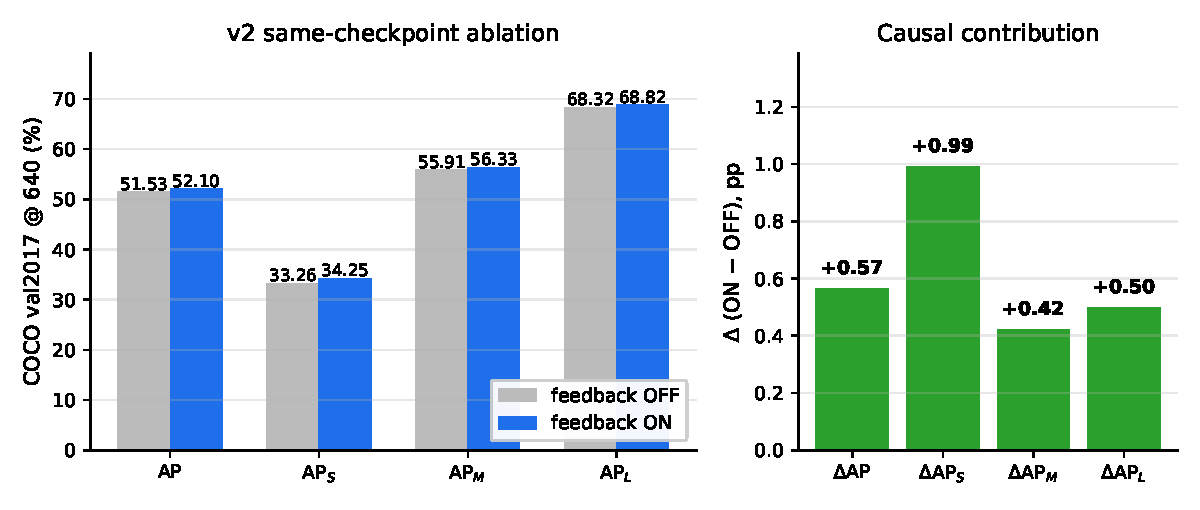
\includegraphics[width=0.95\textwidth]{figures/ablation_bars.pdf}
    \caption{(Left) Absolute v2 scores with feedback OFF (gray) and ON (blue). (Right) The four causal contributions $\Delta = \mathrm{ON} - \mathrm{OFF}$. All four are positive; $\Delta\mathrm{AP}_S = +0.99$ is the largest, in line with the design hypothesis that the gate floor and P2/P3 mask preferentially benefit small-object detection.}
    \label{fig:ablation-bars}
\end{figure}

\subsection{Why this proves causality}

The ablation is a within-run comparison: two evaluations of identical weights, identical inputs, identical inference code except for one Boolean. There is no possibility that "the network learned a stronger backbone path during v2 training and this is what we are measuring" --- such an effect would change OFF too, and it does (v2 OFF = $33.26$ vs v1 OFF = $33.91$, a $-0.65$ drop). The $+0.99$ gap is the contribution that disappears when the feedback computation is skipped, on the same network. v1 had no such gap; v2 does.
